% file: modeledsystems.tex

\chapter{Modeled systems}
This chapter contains descriptions of the systems that I have modeled durung my Master project. 

\section{FCC-lattice (LJ-crystal)}
The FCC-lattice with a Lennard-Jones potential has been extensively investigated due to its simplicity. Therefore it provides robust benchmarking capabilities. Most importantly, I want to check that my protocols for dynamic (but quasistatic) determination of elastic properties and fracture strength reproduces known parameters for a Lennard-Jones solid.
(Poisson ratio 0.347, https://www.researchgate.net/publication/13282313\_Elastic\_compliances\_and\_stiffnesses\_of\_the\_fcc\_Lennard-Jones\_solid)

\section{Bulk S1 hydrate}
\subsection{Elastic properties}
To my knowledge, there are no published estimates of Youngs modulus and the Poisson ratio for the TIP4P/ICE+UAM model of methane hydrates. Therefore, I seek to make crude estimates of these quantities in dynamic simulations. I apply a constant strain rate by continously rescaling particle positions in one direction during MD-simulations. The other directions are kept under a constant pressure with anisotropic barostatting.
Figure \ref{fig:stress_strain_11_11_11_tip4p_ice_uam} shows the stress strain relationships and corresponding estimates of Youngs modulus for a system of 11x11x11 S1 unit cells subjected to strain rates of \SI{5d-7}{\per\femto\second} and \SI{2d-7}{\per\femto\second}. By extrapolating the results to quasistatic strain, Youngs modulus is estimated to \SI{7.1}{\giga\pascal}. 
Figure \ref{fig:strain_strain_11_11_11_y_z_poisson_tip4p_ice_uam} shows the relationship between applied strain along the x-axis and the measured strain along the other axes. It is not outrageous to assume S1 methane hydrate to be isotropic, and under this assumption, extrapolation to quasisatic strain, I estimate the poisson ratio for this model of S1 methane hydrate to be $\nu = 0.41$. 

\begin{figure}
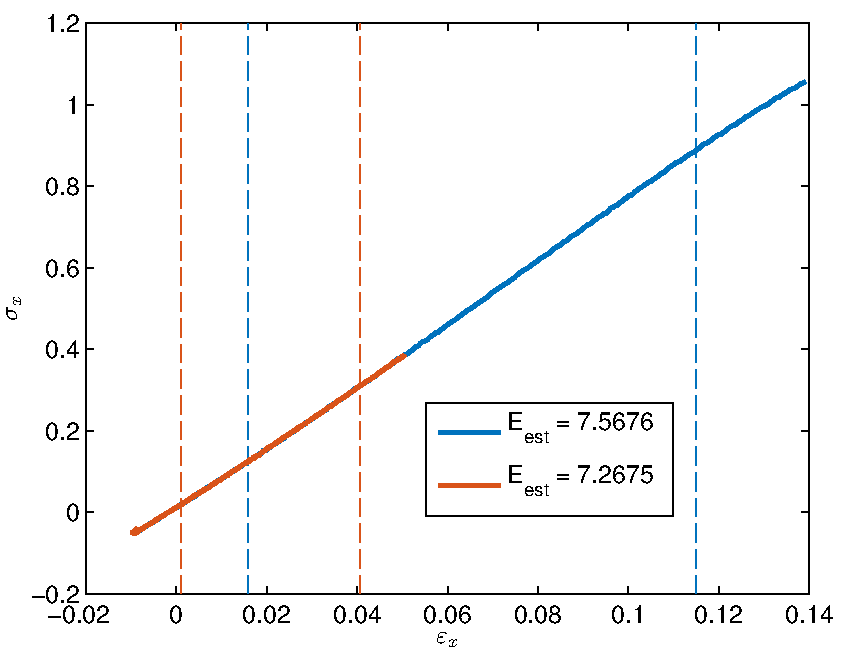
\includegraphics[width=10cm]{../figures/thesis/stress_strain_11_11_11_tip4p_ice_uam.pdf}
\caption{Stess-strain relations for a system of 11x11x11 S1 unit cells. Dashed lines indicate the region that was used to estimate Youngs modulus. Strain rates of \SI{5d-7}{\per\femto\second} (blue) and \SI{2d-7}{\per\femto\second} (red) along the x-axis.}
\label{fig:stress_strain_11_11_11_tip4p_ice_uam}
\end{figure}

\begin{figure}
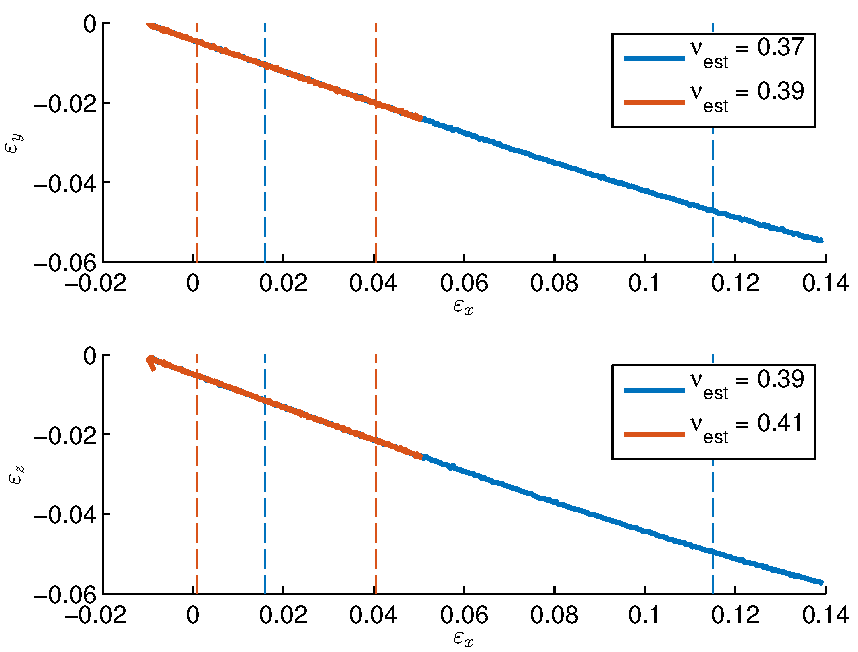
\includegraphics[width=10cm]{../figures/thesis/strain_strain_11_11_11_y_z_poisson_tip4p_ice_uam.pdf}
\caption{Strain-strain relations for the same system as in Figure \ref{fig:stress_strain_11_11_11_tip4p_ice_uam}. Measured strain along the y-axis (a) and z-axis (b) is plotted against the applied strain along the x-axis. Dashed lines indicate the region that was used to estimate Poissons ratio.}
\label{fig:strain_strain_11_11_11_y_z_poisson_tip4p_ice_uam}
\end{figure}

\section{Vega 2010}
\section{Determining the critical stress intensity factor}
As described in the section about fracture mechanics, the stress intensity factor is commonly used to calculate the fracture toughness of a material. Assuming methane hydrates to be brittle (which jush might be a good assumption), I use fracture theories developed by Griffiths to estimate the stress intensity factor for S1 methane hydrate. I cut a 

